% !TEX root =  ../main_manuscript.tex 
\section{Introduction}

Patients with low- and very low-risk screening-detected localized prostate cancer (PCa) are usually advised active surveillance (AS) instead of immediate radical treatment \citep{briganti2018active}. In AS, PCa progression is routinely monitored via prostate-specific antigen (PSA), digital rectal examination, and the Gleason score from repeat prostate biopsies. Among these, the Gleason score is the strongest indicator of cancer related outcomes. Thus, patients are commonly advised curative treatment upon detecting a Gleason score $\geq$ 7 (GS7) \citep{bul2013active}.

Since biopsies are scheduled intermittently, reclassification is always detected with a delay. The smaller this delay is, the larger is the window of opportunity for curative treatment. To this end, majority of the AS programs worldwide, schedule biopsies every 12-24 months for all patients \citep{nieboer2018active,loeb2014heterogeneity}. Such fixed and frequent biopsies may benefit a small proportion of men with a high risk of reclassification. However, for many of the \textit{slow progressing} patients (see Figure \ref{fig:npmle_plot}) frequent biopsies are redundant . Biopsies are also invasive, painful and prone to medical complications. The unnecessary burden of biopsies, and patient non-compliance \citep{bokhorst2015compliance} to frequent biopsies, has raised questions about the optimal time interval between subsequent biopsies \citep{inoue2018comparative, bratt2013study}.

\begin{figure}[!htb]
\centerline{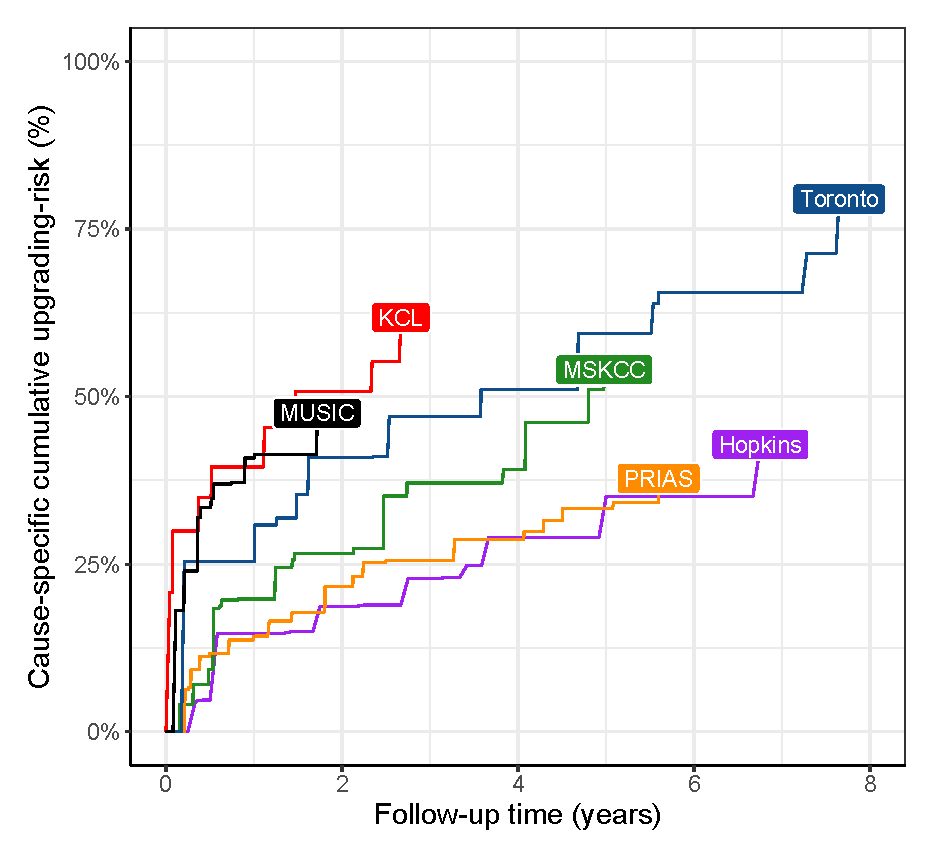
\includegraphics[width=\columnwidth]{images/npmle_plot.eps}}
\caption{\textbf{Active surveillance cancer patients are often \textit{slow progressing}}. Graph shows estimated cumulative risk of having a Gleason score $>$ 6 in five of the largest AS studies that are part of the GAP3 database \citep{gap3_2018}. In all cohorts except KCL, roughly 50\% patients may not require any biopsy in first five years. In the world's largest AS cohort PRIAS and in JHAS, roughly 50\% patients may not require any biopsy in the first ten years. \textbf{Legend}: \textit{JHAS}: Johns Hopkins Active Surveillance, \textit{PRIAS}: Prostate Cancer International Active Surveillance, \textit{Toronto}: University of Toronto Active Surveillance, \textit{MSKCC}: Memorial Sloan Kettering Cancer Center Active Surveillance, \textit{KCL}: King's College London Active Surveillance}
\label{fig:npmle_plot}
\end{figure}

The simplest solution to frequent biopsies is reducing the frequency of biopsies for all patients. However, simulation studies have suggested that reducing the frequency beyond 24 months may not leave sufficient window of opportunity for curative treatment \citep{inoue2018comparative}. Although, even with a gap of 24 months, up to five unnecessary biopsies over ten years of follow-up may still be scheduled for \textit{slow progressing} patients. A promising alternative to such fixed decision of biopsies are the risk based decisions of biopsies. Consider for instance the two patients shown in Figure \ref{fig:riskBasedExample}. Both patients had their latest biopsy at year one of follow-up and are now scheduled for a biopsy after a 24 month gap at year three. The PSA profile of patient A is stable and the PSA profile of patient B is rising. The cumulative risk of reclassification of patient B at year three is also higher than patient A's. Consequently, at year three he is a more suitable candidate for biopsy than patient A.

\begin{figure}[!htb]
\centerline{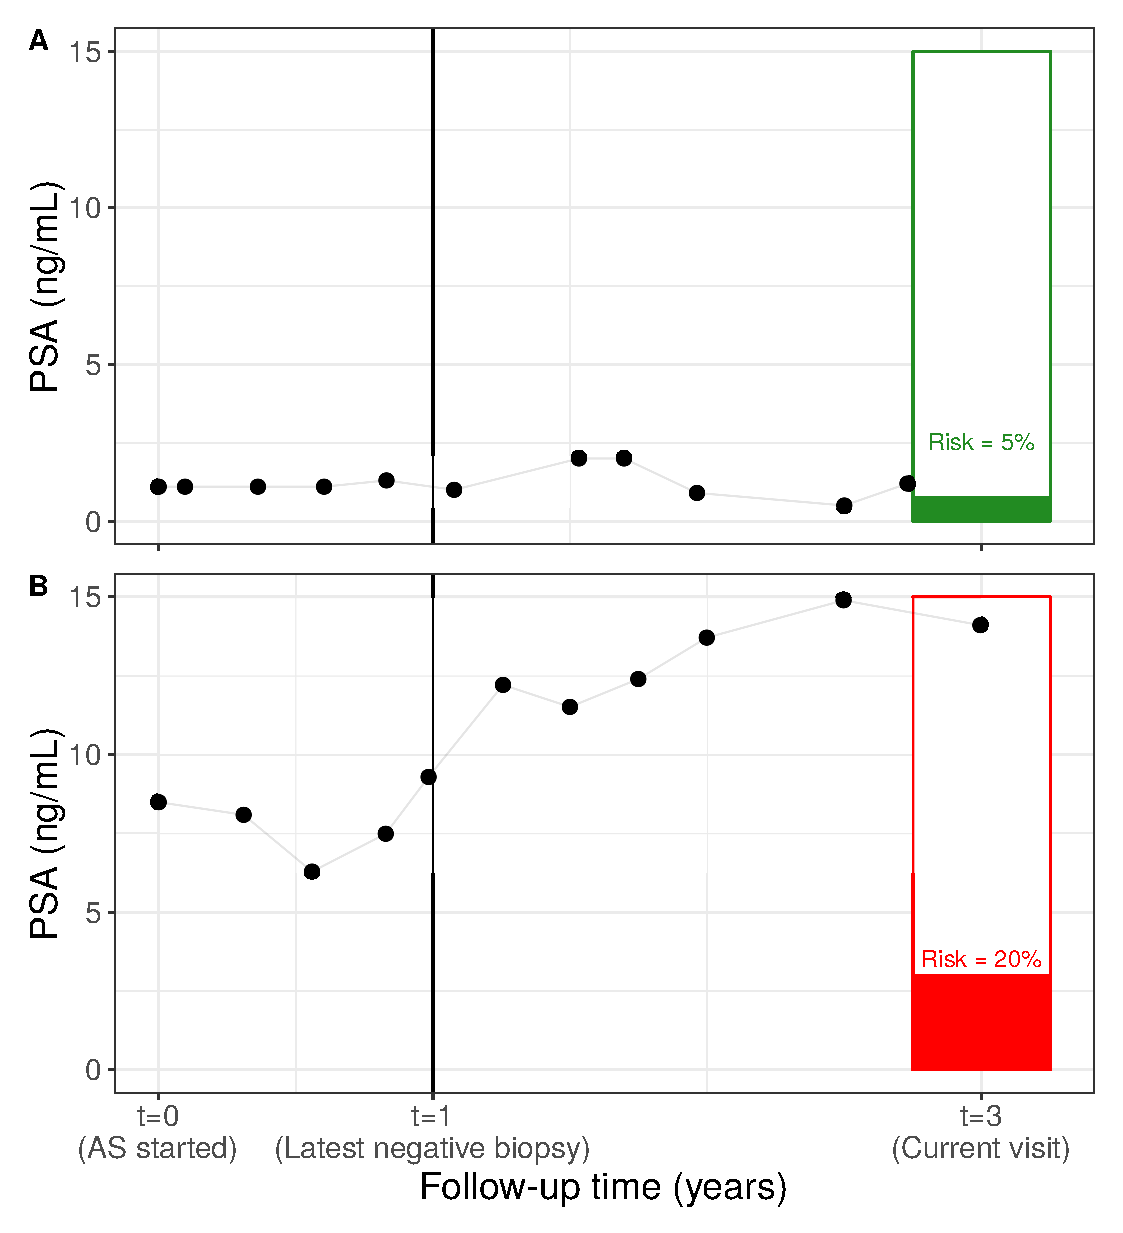
\includegraphics[width=\columnwidth]{images/riskBasedExample.eps}}
\caption{\textbf{Motivation for risk based decisions of biopsy}: Patient A and B had their latest biopsy at year one of follow-up. Patient A's prostate-specific antigen (PSA) profile remained stable until the current visit time at year three. Consequently, his cumulative risk of reclassification at year three is 5\%. On the other hand patient B's PSA profile has shown a rise since the latest biopsy, and his cumulative risk of reclassification is also 20\%. Patient B is a better candidate for biopsy than Patient A.}
\label{fig:riskBasedExample}
\end{figure}

The first challenge in such a risk based approach is the consolidation of observed patient data (e.g., PSA, previous biopsy results) into estimates of the risk of reclassification (Figure \ref{fig:riskBasedExample}). To this end, previous studies have employed joint models for time-to-event and longitudinal data \citep{tomer2019,coley2017prediction,rizopoulos2012joint}. A subsequent challenge however, is to translate these risk estimates into clinical decisions. For example, a 10\% risk can be perceived as high/low depending upon the patient's age. Patients may also weigh the risk of reclassification with the potential consequences of another biopsy. Two such consequences are the delay in detection of reclassification (smaller is beneficial), and the total burden of biopsies. These consequences vary between the patients, and also over the follow-up period for the same patient.

The goal of this work is to assist patients and doctors in making better decisions of biopsies than fixed and frequent biopsies. We intend to achieve this by providing patient- and visit specific risks of reclassification. To further facilitate shared decision making, we also provide estimates of the delay in detection of reclassification and the total burden of biopsies. To this end, we fit a prediction (joint) model to the world's largest AS dataset, PRIAS \citep{bul2013active}. We then validate the predictions in multiple external cohorts that are part of the GAP3 database. Lastly, we implement risk based schedules as a web-application, and demonstrate them with real patient data.